\documentclass[a4paper,anonymous,USenglish]{lipics-v2021} % TODO: Re-add anonymous tag
\usepackage{tikz}

\usepackage{algorithm,algpseudocode}
\algtext*{EndIf}
\algtext*{EndFor}


\theoremstyle{definition}
\newtheorem{construction}{Construction}

\newcommand{\red}[1]{\textcolor{red}{#1}} % TODO: Delete this before submission
\newcommand{\pluseq}{\mathrel{+}=}

\bibliographystyle{plainurl}% the mandatory bibstyle

\title{Relaxation for Efficient Asynchronous Queues}

\titlerunning{Asynchronous Relaxed Queues}

\author{Samuel Baldwin}{Bucknell University, USA}{}{https://orcid.org/0009-0009-0272-759X}{}

\author{Cole Hausman}{Bucknell University, USA}{}{}{}

\author{Mohamed Bakr}{Bucknell University, USA}{}{}{}

\author{Edward Talmage}{Bucknell Univserity, USA}{elt006@bucknell.edu}{https://orcid.org/0009-0001-9108-6190}{}

\authorrunning{S. Baldwin, C. Hausman, M. Bakr, E. Talmage} 

\Copyright{Samuel Baldwin, Cole Hausman, Mohamed Bakr, Edward Talmage} 

\begin{CCSXML}
  <ccs2012>
   <concept>
       <concept_id>10003752.10003809.10010172</concept_id>
       <concept_desc>Theory of computation~Distributed algorithms</concept_desc>
       <concept_significance>500</concept_significance>
   </concept>
   <concept>
       <concept_id>10003752.10003809.10010031</concept_id>
       <concept_desc>Theory of computation~Data structures design and analysis</concept_desc>
       <concept_significance>500</concept_significance>
   </concept>
   <concept>
       <concept_id>10010147.10010919.10010172</concept_id>
       <concept_desc>Computing methodologies~Distributed algorithms</concept_desc>
       <concept_significance>500</concept_significance>
   </concept>
   </ccs2012>
\end{CCSXML}
\ccsdesc[500]{Theory of computation~Distributed algorithms}
\ccsdesc[500]{Theory of computation~Data structures design and analysis}
\ccsdesc[500]{Computing methodologies~Distributed algorithms} %Please choose ACM 2012 classifications from https://dl.acm.org/ccs/ccs_flat.cfm 

\keywords{Distributed Data Structures, Asynchronous Algorithms, Relaxed Data Types}

\funding{Funding provided by Bucknell University}

%\acknowledgements{I want to thank \dots}%optional

%Editor-only macros:: begin (do not touch as author)%%%%%%%%%%%%%%%%%%%%%%%%%%%%%%%%%%
\EventEditors{John Q. Open and Joan R. Access}
\EventNoEds{2}
\EventLongTitle{42nd Conference on Very Important Topics (CVIT 2016)}
\EventShortTitle{CVIT 2016}
\EventAcronym{CVIT}
\EventYear{2016}
\EventDate{December 24--27, 2016}
\EventLocation{Little Whinging, United Kingdom}
\EventLogo{}
\SeriesVolume{42}
\ArticleNo{23}
%%%%%%%%%%%%%%%%%%%%%%%%%%%%%%%%%%%%%%%%%%%%%%%%%%%%%%

\begin{document}
\maketitle

\begin{abstract}
We explore the problem of efficiently implementing shared data structures in an asynchronous computing environment.  We start with a traditional FIFO queue, showing that full replication is possible with a delay of only only two round-trip messages between invocation and response of each operation.  We argue that this is optimal, since any shorter delay would allow scenarios where an algorithm cannot determine correct return values.  We then turn our attention to improving performance.  Here, though we cannot improve the worst-case time per operation instance, we show that \emph{relaxation}, weakening the ordering guarantees of the Queue data type, allows most $Dequeue$ instances to return more quickly than the worst-case, giving a low amortized cost per instance.
\end{abstract}

%%%%%%%%%%%%%%%
%%%%%%%%%%%%%%%
\section{Introduction}

Shared data is a core aspect of modern computing.  Datasets are growing, local computational power cannot keep up, and data collection is continually growing more widespread.  In the naturally resulting geographically distributed systems, one of the primary concerns is accessing data that other members of the system may be accessing concurrently.  Without careful coordination, we can inadvertently use stale versions of the data, overwrite other users' work, or even corrupt the data.

Distributed data structures are a fundamental construct for allowing computing to spread across different machines which need to work together.  By specifying the interface of data operations users may call and the exact effects of those operations, we provide an abstraction layer that allows a programmer designing for a distributed system to not worry about the details of coordinating and maintaining data.  Instead, they can focus on the particular application in which they are interested.  In co-located parallel computation, hardware can exist to provide shared access to memory.  In geographically distributed system, we must build that abstraction layer, considering all the possible oddities of concurrency, messages, delays, and different views of the data.  We focus on optimizing the interactions with these system elements, and provide the developer with an efficient tool which provides well-specified guarantees.

Our primarily concern in this work is to minimize the delays users experience when working with shared data.  Past work has given tight or nearly tight bounds on the possible implementations of a variety of data structures \cite{Kosa99,WangTalmageLeeWelch18} in partially synchronous systems, were there are bounds on the real time which messages between participating processes may take to arrive and processes know and can depend on those bounds.  However, real-world systems do not generally have reliable bounds on timings, so these algorithms are difficult to realistically implement.  As a next step towards practical implementations of efficient distributed data structures, we here consider an asynchronous model of computation.  In this model, processes cannot rely on any local measure of time, or on message delays carrying any information about when remote operations occur, or their order.  Instead, we construct logical timestamps and use them to agree on the order in which operations take place.

This paper contains two results.  First, we present an algorithm for a standard FIFO queue in a fully asynchronous message passing model. While there exist existing solutions for queues in this model \cite{Lynch96}, to our knowledge, none offer full replication, which our solution does.  Replication is important for a few reasons.  First, it enables fault-tolerance, since we do not lose data if a participating system crashes.  We know that asynchronous, fault-tolerant queues are impossible to implement \cite{FischerLynchPaterson85, Herlihy91}, so we cannot immediately proceed to adding fault tolerance to this algorithm.  There are other benefits of replication, though, such as data locality and not relying on a central coordinating process, which may be subject to malicious control.  Our main purpose in relaxation is to support our second result, which may be able to avoid previous impossibility results and lead to future fault-tolerant data structures.

Our second result builds on the notion of \emph{relaxing} a data type: weakening the guarantees of the data type specification \cite{HenzingerKirschPayerSezginSokolova13}.  We can then use this weakening to achieve better performance than we can for a basic data type.  Following Talmage and Welch \cite{TalmageWelch14}, we consider a version of a Queue datatype that allows $Dequeue$ to return not just the single oldest element, but any sufficiently old element in the structure.  This allows us to determine return values for most $Dequeue$ invocations without waiting for any communication, thus bringing the amortized cost of $Dequeue$ far below the minimum possible for an unrelaxed queue.  We provide an algorithm doing this, building on our first algorithm.  This algorithm is the first to implement a relaxed queue in an asynchronous system and proves that the performance benefits Talmage and Welch \cite{TalmageWelch14} found in partially synchronous systems are also possible in asynchronous systems.  While the relaxed queue does not provide the same ordering guarantees as a FIFO queue, in many concurrent executions, the behavior will be indistinguishable.  If a process dequeues, for example, the third oldest element in the queue, this appears similar (at least at that time), to an execution of an unrelaxed queue where two other processes concurrently dequeued the two older elements, as this process will still dequeue the third oldest element.

Another intriguing property of relaxed queues is that they are not as subject to the impossibility results for asynchronous, fault-tolerant systems \cite{ShavitTaubenfeld16,TalmageWelch19}.  Thus, it may well be possible to extend our result in the future to asynchronous, fault-tolerant implementations.  This would be a major step forward, since the impossibility of implementing queues, and most other useful data types severely limits the capabilities of distributed systems.  This paper is a step on the road toward that goal, and we are excited to pursue such implementations.

%and therefore the ability to extend to fault tolerant systems. Our algorithm utilizes vector clock timestamps that allow individual processes to hold some view of the time steps of other processes have taken at points of communication. Using this technique to timestamp invocations of the two operations of the queue, then linearizing all of the queue invocations based on the ascending lexicographic order of these timestmps creates a valid permutation that meets the specifications of a FIFO Queue.  The goal of establishing this queue method is to design a system with full replication. There are existing systems that handle the asynchronous queue (server client model), but are incapable of replication. With replication, and (INSERT THE CITATION TO THE PAPER HERE) we hope that this queue algorithm can be used in fault tolerant systems in the future.

%%%%%%%%%%%%%%%
\subsection{Related Work}

TODO

% Lamport: Linearizability, data structure implementations
% ABD: Register implementations in asynchronous systems

% Relaxation:
% Afek et al. Quasi-linearizability
% Henzinger et al. Quantitative relaxation
% Talmage Welch '14 improving data structure performance

% Computational power
% FLP, Herlihy
% Shavit Taubenfeld/TalmageWelch19: lower CNs for relaxed queues

%%%%%%%%%%%%%%%
%%%%%%%%%%%%%%%
\section{Model and Definitions}

%%%%%%%%%%%%%%%
\subsection{Asynchronous System Model}
We assume a fully asynchronous message passing model of computation.  The system contains a set of $n$ processes $\Pi = [p_0, \dots , p_{n-1}]$ modeled as state machines, and a set of $n$ users, one for each process.  Each state machine accepts two types of inputs: the corresponding user may \emph{invoke} an operation, or the machine may \emph{receive} a message.  Each of these will trigger a handler.  Each process, in its handlers, may perform local computation, or perform one of of two external actions: it may \emph{respond} to its user or \emph{send} a message to another process.  The state machines are time-free, meaning that their output is only described through their input and state transitions without any specific time bound.  We also assume no processes fail, instead performing exactly as per the state machine specification.  

We assume all inter-process communication is reliable, so when a process sends a message, that message will eventually be received at its destination process exactly once.  Additionally, we assume communication channels between processes are First-In, First-Out.  That is, if process $p_i$ sends message $m_1$ to process $p_j$, then sends message $m_2$ also to $p_j$, then $p_j$ will receive $m_1$ before it receives $m_2$.  This assumption does not reduce the generality of our results, as we can implement such an ordering guarantee by attaching a sequence number to each message and buffering incoming messages at each process.  We store out of order messages in this buffer until all previous messages are received, then receive the buffered message.

%TODO: expand definition of reliable channels to mention messages arrive in finite time

While there is no notion of time available to processes in the system, we establish a notion of the time cost of our algorithms by considering that they run in real time.  There are no upper or lower bounds on either local computation time or the time between when a message is sent and received.  However, we can measure an algorithmic time, from outside the system, by expressing it in terms of the number of sequential messages which must occur in that duration \cite{AttiyaWelch04}.  That is, in a particular run, we define the parameter $d$ as the real time duration of the longest time between sending and receiving any one message.  We express algorithmic time in terms of $d$, by considering how many messages the algorithm sends and receives, with each send necessarily occurring after the receive of the previous message.  Since each of those delays may be the largest in that run, this gives a measure of algorithmic runtime without bounding real time message delays.  

%%%%%%%%%%%%%%%
\subsection{Data Type Definitions}

We first state the definition for a standard FIFO queue abstract data type, then that for the relaxed queue we study here.  We state abstract date type (ADT) specifications in two parts: First, a list of operations the user can invoke, with argument and return types, expressed as $OP(arg,ret)$.  We use $-$ to indicate when a function takes no argument or returns no value.  Second, we define the set of legal \emph{instances} of these operations.  An operation instance is an invocation-response pair, noting that these are significantly separate events in a distributed setting.  We assume that each process' user cannot invoke an operation until it has received a response to its last previous invocation.   

To simplify the statement of our definitions, we assume that each argument to $Enqueue$ is unique.  One way to achieve this practically would be a simple abstraction layer that adds a (logical) timestamp to each value before it is passed to the data structure.  We also define the notion of \emph{matching}: A $Dequeue$ instances matches an $Enqueue$ instance if it returns that $Enqueue$'s (unique) argument.  We will use the special character $\bot$ to represent an empty queue.

\begin{definition}\label{def:FIFOQueue}
  A \emph{Queue} over a set of values V is a data type with two operations:
  \begin{itemize}
  \item $Enqueue(val,-), val \in V$ 
  \item $Dequeue(-, val), val \in V \cup \{\bot\}$ 
  \end{itemize}
  
  The empty sequence is legal.  For any legal sequence $\rho$ of instances of queue operations and $val \in V$, (1) $\rho \cdot Enqueue(val,-)$ is legal, (2) $\rho \cdot Dequeue(-,val)$ is legal iff $Enqueue(val, -)$ is the first unmatched $Enqueue$ instance in $\rho$, and (3) $\rho \cdot Dequeue(-, \bot)$ is legal iff every $Enqueue(val, -)$ in $\rho$ is matched.
\end{definition}

We can now formally define the relaxed queue we implement in this paper.  Intuitively, each $Dequeue$ instance can return one of the $k$ oldest elements in the queue.  If $k=1$, this is the same as the FIFO Queue defined above.

\begin{definition} A \emph{Queue with $k$-Out-of-Order relaxed $Dequeue$}, or an \emph{$k$-Out-of-Order Queue}, over a set of values $V$ is a data type with two operations:
  \begin{itemize}
  \item $Enqueue(val,-), val \in V$
  \item $Dequeue(-,val), val \in V$
  \end{itemize}

  The empty sequence is legal.  For any legal sequence $\rho$ of instances of $k$-out-of-order queue operations and $val \in V$, (1) $\rho \cdot Enqueue(val,-)$ is legal, (2) $\rho \cdot Dequeue(-,val)$ is legal iff $val$ is the argument of one of the first $k$ unmatched $Enqueue$ instances in $\rho$, and (3) $\rho \cdot Dequeue(-,\bot)$ is legal iff there are fewer than $k$ unmatched $Enqueue$ instances in $\rho$.
\end{definition}

We are interested in implementations which satisfy \emph{linearizability} \cite{HerlihyWing90}.  Linearizability is a consistency condition which describes how concurrent executions of a data structure relate to the sequential specification of the ADT the structure implements.  Specifically, linearizability requires that operation response values be such that there is a total order of all operation instances in the execution which is legal according to the ADT and which respects the real-time order of instances which do not overlap in real time.  That is, if one instance returns before, in real time, another's invocation, that one which returned first must be ordered first.  This condition provides behavior that matches that we intuitively expect systems to have, disallowing inversions in real time.  Linearizability also has the advantage of being composable, meaning that running multiple linearizable objects in the same execution will necessarily produce an overall linearizable execution.  Linearizability is the strongest consistency condition we might satisfy, so our upper bounds translate to any other consistency condition one might use.

% TODO: Define run, timed run, admissible (must be infinite), linearization, single pending instance per process

%%%%%%%%%%%%%%%
%%%%%%%%%%%%%%%
\section{Asynchronous FIFO Queues}

%%%%%%%%%%%%%%%
\subsection{Description}

TODO: Write high-level description of algorithm. (broadcasts, confirmations/conflists, local copy of the queue and local execution, etc.).  Don't put a lot of detail here, as we'll expand on those below.

%%%%%%%%%%
\subsubsection{Vector Clocks}

Each process stores a vector clock timestamp that holds its local view of the clocks at all processes.  We will refer to the local vector clock at process $p_i$ as $v_i$.  Each process' vector clock is an array of size $n$ that is initially 0 at all indices.  When any process $p_i$ invokes $Enqueue$ or $Dequeue$, $p_i$ will increment index $i$ in its local clock, $v_i[i]$.  Processes also update the local view of the vector clocks when they receive a message containing a timestamp from another process.  Each invocation of $Enqueue$ or $Dequeue$ sends a timestamp, as well as other messages our algorithm uses for coordination.  To update its local vector clock, the receiving process compares values at corresponding indexes of the local clock and received timestamp, and sets its local clock at that index to the larger of the two values.  By adjusting each of these indices, this guarantees that a local clock will have the largest of the two indices at all indices in the local clock, recording its knowledge of the previous remote event for all later timestamps.

We define two orders on timestamp vectors.  For any two vector timestamps $v_i$ and $v_j$, we say $v_i$ is \emph{strictly smaller} than $v_j$, denoted $v_i \prec  v_j$, if $v_i[x] < v_j[x],\forall x \in [0, \dots, n-1]$.  If this is not true, there is some index $k$, where the vectors first differ.  That is, for $x = 0$ to $k-1$, $v_i[k] < v_j[x]$ but $v_i[k] \geq v_j [k]$.  Then we say that $v_i$ is \emph{lexicographically smaller} than $v_j$ and write $v_i << v_j$.  Notice that $v_i \prec v_j$ implies that $v_i << v_j$ but not the opposite.

Each process maintains a local augmented minimum priority queue keyed on lexicographic timestamp order.  This priority queue can perform three operations: $insert(value, v_{clock})$, $get(position)$, and $remove(value)$.  The $insert$ operation adds the value to the queue with $v_{clock}$ as a priority.  The $get(position)$ function allows the user to peek into the element at the passed position (returns the element with the $position$th-lowest timestamp) without removing a value from the queue.  The $remove(value)$ function removes the specific value passed to it from the queue, independent of priority order.  Ordering elements in FIFO order is not a straight-forward task in a distributed setting since defining which invocation happened first is well defined for concurrent operation instances.  We will use lexicographic timestamp order for our linearization, so using a priority queue keyed on lexicographic timestamp order allows us to ensure each process' local view matches that of the linearization order.

%%%%%%%%%%
\subsubsection{Confirmation Lists}\label{sec:confLists}
The main algorithmic idea that allows us to handle asynchrony is a structure we call \emph{Confirmation Lists}.  Each process uses these lists to track acknowledgments from other processes for a given $Dequeue$ instance.  When aprocess $p_j$ receives a $Dequeue$ request message from another process $p_i$, $p_j$ will either declare that $Dequeue$ instance $unsafe$ or $safe$ depending on whether $p_j$ has or has not, respectively, invoked a $Dequeue$ intance with smaller (lexicographically)\footnote{\textcolor{red}{TODO: make sure I got the right ordering here}} timestamp.  $p_j$ will then send a its response to all processes, declaring its view of the $Dequeue$ instance as $safe$ or $unsafe$. These $safe$/$unsafe$ messages also contain the invoking process's id, the responding process' id, and the invocation's vector clock timestamp.  \textcolor{red}{TODO: mention invoation timestamps earlier somewhere}  The idea is that, if $p_j$ is already dequeueing, it will mark $p_i$'s $Dequeue$ as $unsafe$ and broadcast this, to ensure that all processes execute $p_j$'s $Dequeue$ instance on their local copy before $p_i$'s $Dequeue$ instance.

To track these $safe$/$unsafe$ responses, when a process first receives information about a $Dequeue$ invocation, it creates a \emph{confirmation list} object, keyed to the timestamp of the $Dequeue$ invocation and stores that object.  This object contains the timestamp that distinguishes it from other confirmation lists, then an array of length $n$, to track confirmations from each process.  A process can learn about an invocation by invoking a $Dequeue$ itself, from a $Dequeue$ request message directly from the invoking process, or from a third-party process' response message to a $Dequeue$ invocation.  A confirmation list's array is empty at creation, except for a $safe$ in the position corresponding to the invoking process.  The list fills as the process receives $safe$/$unsafe$ responses to the $Dequeue$ request, placing each in the position corresponding to the responding process.  If a process is creating a confirmation list on receiving a response before the initial $Dequeue$ request, it can place that response in the position corresponding to the sender immediately on creating the confirmation list.

If process $p_j$ is storing a confirmation list for a $Dequeue$ instance invoked at process $p_i$, when the confirmation list's array has no empty cells because it has received responses from all processes, $p_j$ can locally execute that $Dequeue$ instance, applying it to its own local copy of the queue.  To ensure that it removes the same element as all other processes, $p_i$ counts the number of $unsafe$ responses stored in the instance's confirmation list and uses that as the $position$ argument to a $get$ call.  Each $unsafe$ corresponds to another, concurrent $Dequeue$ instance which has a lexicographically smaller timestamp, and which thus will be linearized earlier.  Thus, the algorithm uses the $get$ function to leave the elements those preceding $Dequeu$ instances wll return.

At the point of locally executing a $Dequeue$ instance via the confirmation list structure, any other confirmation lists for $Dequeue$ instances with lexicographically later timestamps must be updated, since they no longer need to save an element for the already-executed instance.  The invoking process for the executed $Dequeue$ instance would have responsed with $unsafe$ to any $Dequeue$ requests during the period between when invoking $Dequeue$ and when it locally executes it.  When $p_j$ locally executes the invocation, it removes the element that the process is effectively reserving with the $unsafe$ responses. Therefore, we can change to $safe$ all responses $p_i$ sent as $unsafe$ while its $Dequeue$ instance was pending.  To do this, $p_j$ will update confirmation lists stored for $Dequeue$ instances with lexicographically later timestamps, changing any $unsafe$ values in the position corresponding to $p_i$ to $safe$.  This updating stops at the next confirmation list for a $Dequeue$ instance invoked at process $p_i$, as any $unsafe$ responses $p_i$ sent after that point will be because this next $Dequeue$ instance was pending, instead of because of the original instance.

%%%%%%%%%%%%%%%
\subsection{Algorithm}

This algorithm is based on that of Talmage and Welch \cite{TalmageWelch14}.  Instead of using timers based on knowledge of message delays, we here use round-trip messages to indicate when processes can apply operation instances to their local replicas of the shared queue.  As discussed, we also use vector clocks to order events.

We first outline a number of local variables and sequential functions used by our local data structures.  We discussed $PendingDequeues$ and confirmation lists, in Section~\ref{sec:confLists} above.
\begin{itemize}
\item $v_i$: Process $p_i$'s vector clock, an array with one entry for each process.
\item $lQueue$: Each process' local replica of the shared queue.
\item $lQueue.insertByTS(val, inv, ts)$: Adds an entry to $lQueue$, sorting by lexicographic timestamp order on $ts$, and saving the value $val$ along with $ts$ and the invoking process id $inv$.
\item $lQueue.dequeue(ts)$: Returns and removes the oldest element in $lQueue$ with timestamp smaller than $ts$, $\bot$ if there is none.
\end{itemize}
% TODO: Define variables, structures, functions.
% Specifically: 

\begin{algorithm}
  \caption{Code for each process $p_i$ to implement a Queue}\label{alg:fifo}
  \begin{algorithmic}[1]
    \Function{Enqueue}{$val$}\label{fifoline:invEnq}
      \State $EnqResponseCount = 0$ \Comment{Count responses to this invocation}
      \State $Enq_{ts} = updateTS()$ \label{fifoline:enqTS} \Comment{Increment local vector clock, read instance's timestamp}
      \State send $(EnqReq, val, Enq_{ts}, i)$ to all processes\label{fifoline:sendEnqReq}
    \EndFunction

    \Function{Receive}{$EnqReq, val, inv, Enq_{ts}$} from $p_{inv}$
      \State $updateTS(Enq_{ts})$ \label{fifoline:enqReqTSUpdate} \Comment{Update local vector clock by invocation's timestamp}
      \State $lQueue.insertByTS(val, inv, Enq_{ts})$\label{fifoline:executeEnq} \Comment{Locally execute the $Enqueue$ instance}
      \State send $(EnqAck, i)$ to $p_{inv}$ \label{fifoline:sendEnqAck} \Comment{Acknowledge receipt of the invocation}
    \EndFunction

    \Function{Receive}{$EnqAck, j$ from $p_j$}
      \State $EnqResponseCount \pluseq 1$
      \If {$EnqResponseCount == n$} 
        \Return $EnqResponse$ to user\label{fifoline:enqReturn} 
      \EndIf
    \EndFunction \label{fifoline:finishEnq}
%
    \Function{Dequeue}{}
      \State $Deq_{ts} = updateTS()$ \Comment{Increment local vector clock, read instance's timestamp}\label{fifoline:deqTS}
      \State send $(DeqReq, Deq_{ts}, i)$ to all processes \label{fifoline:sendDeqReq}
    \EndFunction
%
    \Function{Receive}{$(DeqReq, Deq_{ts}, inv)$ from $p_{inv}$}
    \State $updateTS(Deq_{ts})$ \label{fifoline:deqReqTSUpdate}
      \If{$Deq_{ts}$ is not in $PendingDequeues$}
      \State $PendingDequeues.insertByTS(createList(Deq_{ts}, p_{inv}$))\label{fifoline:savePendingDeq}
      \EndIf
      \State send $(DeqAck, Deq_{ts}, p_{inv}, i)$ to all processes \label{fifoline:sendSafetyFlag}\label{fifoline:sendDeqAck}
    \EndFunction
%
    \Function{Receive}{$(DeqAck, Deq_{ts}, p_{inv}, j)$ from $p_j$}
      \If{$Deq_{ts}$ not in $PendingDequeues$}
        \State $PendingDequeues.insertByTs(createList(Deq_{ts}, p_{inv}))$
      \EndIf
      \State Define $currentConfList$ as the confirmation list in $PendingDequeues$ which has $ts == Deq_{ts}$
      \State $currentConfList.responses[j] = True$ \label{fifoline:setResponse}
      \State $propagateEarlierResponses(PendingDequeues, Deq_{ts}, j)$ \label{fifoline:propagateEarlier} \Comment{Enable lower-timestamp pending $Dequeue$ instances to execute}

      \For{each $confirmationList$ in $PendingDequeues$, in increasing lexicographic timestamp order}
        \If{all $response$s in $confirmationList$ are $True$}\label{fifoline:fullConfList}
          \State $ret = lQueue.dequeue(Deq_{ts})$\label{fifoline:chooseDeqValue} \Comment{Locally execute the $Dequeue$ instance, ignoring elements with later timestamps} 
        \State delete $confirmationList$ from $PendingDequeues$
        \If{$p_i == p_{inv}$} \Return $ret$ to user \label{fifoline:deqReturn} \EndIf \Comment{The invoking process responds to the user}
      \EndIf 
      \EndFor

      \EndFunction
      \Statex
      \Statex \emph{(continues below)}

    \algstore{fifoLines}  
  \end{algorithmic}
\end{algorithm}

\begin{algorithm}[t]
  \caption{Algorithm~\ref{alg:fifo} continued: Helper functions}
  \begin{algorithmic}[1]
    \algrestore{fifoLines}
    
    \Function{propagateEarlierResponses}{$PendingDequeues, Deq_{ts}$}
      \Statex \Comment{If a later-timestamp instance receives a $DeqAck$, then any earlier-timestamp instances need wait no longer for a $DeqAck$ from that process.}
      \For{each confirmation list $PendingDequeues[j]$, in decreasing timestamp order} 
        \For{each process id $k$}
          \If{$PendingDequeues[j].responses[k]$ and $j>0$}
            \State $PendingDequeues[j-1].responses[k] = True$
          \EndIf
        \EndFor
      \EndFor  
    \EndFunction
%
    \Function{updateTS}{$v_j$}
      \If{$v_j$ is empty}
        \State $v_i[i] \pluseq 1$
      \Else
        \For{$k = 0$ up to $n - 1$}
          \State $v_i[k] = max(v_i[k], v_j[k])$
        \EndFor
      \EndIf
      \State return $v_i$
    \EndFunction
%
    \Function{createList}{$Deq_{ts}, p_{invoker}$}
      \State create a new confirmation list $ConfirmationList$
      \State $ConfirmationList.responses = [0,0,...,0]$ \Comment{An array of $n$ 0s}
      \State $ConfirmationList.ts = Deq_{ts}$ \Comment{A vector clock timestamp}
      \State $ConfirmationList.invoker = p_{invoker}$ \Comment{The invoking process of the Dequeue}
      \State return $ConfirmationList$
    \EndFunction
  \end{algorithmic}
\end{algorithm}


%%%%%%%%%%%%%%%
\subsection{Correctness}\label{sec:fifoCorrectness}
In order to prove that this algorithm correctly implements the queue specification, we will consider an arbitrary, admissable timed run $R$.  We will first prove that all invocations have a matching return, so that we have complete operation instances.  We can then construct a total order of all operation instances in $R$ and prove that it respects real time order, making it a valid linearization, and is legal by the specification of a queue.  The core of the proof is in proving that when any process removes a particular $Dequeue$ instance's return value from its local replica of the queue, it deletes the same value as every other process does.  This means that all replicas will undergo the same series of operations, and allows us to prove that they continue removing the correct values.  To ensure that all processes remove the same element, we use the $safe$/$unsafe$ flags to leave elements for any $Dequeue$ instances which linearize earlier, but which that process is not ready to execute on its replica.

\begin{lemma}\label{fifolem:responses}
  In $R$, every invocation has a matching response.
\end{lemma}

\begin{proof}
When a user invokes an operation at process $p_i$, the algorithm sends an $EnqReq$ message containing the invocation to all processes on line~\ref{fifoline:sendEnqReq} or \ref{fifoline:sendDeqReq}, depending on the operation invoked.  Each process will receive that message in finite time by our assumption of reliable channels and send back an $EnqAck$ for an $Enqueue$ invocation on line~\ref{fifoline:sendEnqAck} or a safety flag for a $Dequeue$ invocation on line~\ref{fifoline:sendSafetyFlag}, as appropriate.  Each of those responses will arrive in finite time, and when $p_i$ receives all $n$ of them, it will generate a matching return on line~\ref{fifoline:enqReturn} for $Enqueue$ or line~\ref{fifoline:deqReturn} for $Dequeue$.
\end{proof}

Each process reads its vector clock at each invocation, on line~\ref{fifoline:enqTS} or \ref{fifoline:deqTS}, and associates that clock value with that invocation throughout the algorithm.  We will refer to this clock value as the \emph{timestamp} of the instance containing that invocation.

\begin{construction}\label{constr:fifo}
  Let our linearization $\pi$ be the increasing lexicographic order of all operation instances in $R$.
\end{construction}

\begin{lemma}\label{fifolem:realTimeOrder}
  $\pi$ respects the real time order of non-overlapping instances.
\end{lemma}
\begin{proof}
  Proof by contradiction. Let there be two non-overlapping operation instances $op_1$ and $op_2$, where $op_1$ returns prior to $op_2$'s invocation in real time.  Assume, for the sake of contradition, that $op_2$ is prior to $op_1$ in $\pi$.
  
  Given that $op_1$ occurs before $op_2$ in real time, and that the two operation instances are non-overlapping, $op_2$'s timestamp must be larger, lexicographically, than $op_1$'s.  This follows from the fact that $op_1$ will not return until it receives a response from every process, including $op_2$'s invoking process (lines~\ref{fifoline:enqReturn}, \ref{fifoline:deqReturn}.  This means that $op_2$'s invoking process received the invocation for $op_1$ and updated its timestamp (line~\ref{fifoline:enqReqTSUpdate} or \ref{fifoline:deqReqTSUpdate}) before it invoked $op_2$, so $op_2$'s timestamp will be totally ordered after $op_1$'s, implying it is also lexicographically after.
\end{proof}

Next, we consider how each process locally executes each $Dequeue$ instance.  We show that all processes do so in the same way, meaning that their replicas of the data structure move through similar sequences of states, and thus continue to behave properly.  Processes may locally execute $Enqueue$ instances at different times, but since we store those instances' timestamps with the values in the local replicas, we will never delete a value from an $Enqueue$ intance later in the linearization.

\begin{lemma}\label{fifolem:prevLocalExec}
  When a process $p_i$ locally executes any $Dequeue$ instance $op$, for any instance $op'$ with a lexicographically smaller timestamp than $op$, $p_i$ has previously locally executed $op'$.
\end{lemma}

\begin{proof}
  By line~\ref{fifoline:fullConfList}, $p_i$ will not locally execute $op$ until it has received a $DeqAck$ for $op$ from every process, either for $op$ or for a $Dequeue$ instance with larger timestamp than $op$ (line~\ref{fifoline:propagateEarlier}).  But when any process sends a $DeqAck$, on line~\ref{fifoline:sendDeqAck}, it has updated its timestamp to be larger than $op$'s timestamp.  Thus, any instance invoked at that process after that point will have a totally, and thus lexicographically, larger timestamp than $op$.  This means that any instance $op'$ invoked at $p_j$ with a lexicographically smaller timestamp than $op$ must have been invoked before its invoking process sent a $DeqAck$ for $op$ or any later $Dequeue$ instance.

  By FIFO message order, $p_j$'s request message for $op'$, which it sends on line~\ref{fifoline:sendEnqReq} or \ref{fifoline:sendDeqReq}, would have arrived at $p_i$ before the $DeqAck$ for $op$ from $p_j$, and $p_i$ would have either locally executed $op'$ on line~\ref{fifoline:executeEnq} if it was an $Enqueue$ instance, or put it in $PendingDequeues$ on line~\ref{fifoline:savePendingDeq} if it was a $Dequeue$ instance.  If it was a $Dequeue$ instance, the only time $p_i$ could remove $op'$ from $PendingDequeues$ is in lines~\ref{fifoline:fullConfList}-\ref{fifoline:deqReturn}, when $p_i$ locally executes $op'$.  Thus, when $p_i$ locally executes $op$, it must have already either locally executed $op'$, or have it in $PendingDequeues$.

  But $p_i$ can only locally execute $op$ when its confirmation list is full, and any time $p_i$ sets a response entry in $op$'s confirmation list to true on line~\ref{fifoline:setResponse}, it then propagates responses to all pending $Dequeue$ instances with smaller timestamps on line~\ref{fifoline:propagateEarlier}.  Thus, if $p_i$ has received a response from every process for $op$, it has also marked every $response$ cell in the confirmation list for $op'$, and will locally execute $op'$ before $op$.
\end{proof}

This means that during local execution of a $Dequeue$ instance, each process has already placed the arguments of all earlier-linearized $Enqueue$ instances in its replica of the queue and has already locally executed every $Dequeue$ instance with a smaller timestamp.  

\begin{corollary}\label{fifolem:localExecOrder}
  Each process locally executes all $Dequeue$ instances in increasing lexicographic timestamp order.
\end{corollary}

\begin{lemma}\label{fifolem:legal}
  $\pi$ is a legal sequence by the specification of a FIFO queue.
\end{lemma}

\begin{proof}
  We prove this claim by induction on $\pi$.  The empty sequence is legal.  Assume that in any prefix $\rho \cdot op$ of $\pi$, $\rho$ is legal.  We will show that $rho \cdot op$ is also legal which, by induction, implies that $\pi$ is legal.  Let $p_i$ be the process which invoked $op$.

  If $op$ is an $Enqueue$ instance, then $\rho \cdot op$ is legal by Definition~\ref{def:FIFOQueue}.

  If $op$ is a $Dequeue$ instance, $op = Dequeue(-,ret)$, we must show that either $ret \neq \bot$ is the argument of the first unmatched $Enqueue$ instance in $\rho$ or there $ret = \bot$ and there are no unmatched $Enqueue$ instances in $\rho$.

  We begin with the case that $ret \neq \bot$.  This means that when $p_i$ chose $ret$ as the return value in line~\ref{fifoline:chooseDeqValue}, it found $ret$ in its local replica of the queue, with timestamp lexicographically less than $ts(op)$.  Thus, $ret$ was the argument of some $Enqueue$ instance in $\rho$, since the only values added to an $lQueue$ are $Enqueue$ arguments, in line~\ref{fifoline:executeEnq}.

  We next prove that $Enqueue(ret,-)$ is the first unmatched $Enqueue$ instance in $\rho$.  By Lemma~\ref{fifolem:prevLocalExec}, when $p_i$ locally executes $op$ and chooses its return value, it has already locally executed every $Enqueue$ instance with a lexicographically smaller timestamp.  By Construction~\ref{constr:fifo}, these are the $Enqueue$ instances in $\rho$.  Thus, the set of elements $p_i$ has available to choose are the arguments of $Enqueue$ instances in $\rho$.  Further, by Corollary~\ref{fifolem:localExecOrder}, $p_i$ has locally executed every $Dequeue$ instance with timestamps smaller than $op$, which is exactly those $Dequeue$ instances in $\rho$.

  Thus, $p_i$'s $lQueue$ contains exactly the arguments of unmatched $Enqueue$ instances in $\rho$, as well as potentially the arguments of some $Enqueue$ instances which appear in $\pi$ after $op$.  Line~\ref{fifoline:chooseDeqValue} chooses the value in $lQueue$ with the smallest timestamp, filtering to only those with timestamp smaller than $op$, which is the argument of the first unmatched $Enqueue$ instance in $\rho$, since we constructed $\rho$ in timestamp order.  Similarly, when any other process locally executes $op$, they will delete the same value from their $lQueue$ by the same logic, simply not returning it to their user by the check on line~\ref{fifoline:deqReturn}.  

  The next case we consider is when $ret = \bot$.  In this case, when $p_i$ executes line~\ref{fifoline:chooseDeqValue}, it finds no element in $lQueue$ with smaller timestamp than $op$.  By the logic in the previous case, this means that every $Enqueue$ instance with timestamp smaller than $op$ is matched by a $Dequeue$ instance in $\rho$, so $\rho \cdot op$ is legal.

  Thus, by induction, $\pi$ is legal.
\end{proof}


\begin{theorem}
  Algorithm~\ref{alg:fifo} correctly implements a FIFO queue.
\end{theorem}

\begin{proof}
  By Lemma~\ref{fifolem:realTimeOrder}, $\pi$ respects the real-time order of non-overlapping instance and by Lemma~\ref{fifolem:legal}, $\pi$ is a legal sequence of operation instance on a FIFO queue.  Thus, every run $R$ of Algorithm~\ref{alg:fifo} has a valid linearization, so it is a correct implementation.
\end{proof}
 

%%%%%%%%%%%%%%%
\subsection{Complexity}

As observed in Lemma~\ref{fifolem:responses}, the algorithm returns to every invocation after it receives acknowledgements from every other process.  This takes up to $2d$ time, since the request message must reach each other process before they can send the acknowledgement, and the two non-concurrent messages can each take up to $d$ time.

This runtime is optimal, as we can show by a simple indistinguishability argument, that any \emph{pair-free} operation must take at least $2d$ time from invocation to response.  A pair-free operation \cite{WangTalmageLeeWelch18} is one, like $Dequeue$, which both depends on and changes the state of the data structure, such that it is possible for a pair of adjacent instances to not be legal in reverse order.  For example, $Enqueue(1) \cdot Dequeue(1)$ is legal, but $Enqueue(1) \cdot Dequeue(1) \cdot Dequeue(1)$ is not, because the first $Dequeue$ instance changed the state of the structure.  Formally, there exist a legal sequence $\rho$ and two (not necesssarily distinct) instances $op_1, op_2$, such that $\rho \cdot op_1$ and $\rho \cdot op_2$ are both legal, but $\rho \cdot op_1 \cdot op_2$ and $\rho \cdot op_2 \cdot op_1$ are not both legal.

\begin{lemma}\label{fifolem:pairfreeLB}
  The worst-case cost of $Dequeue$ in our asynchronous, failure-free message passing model is at least $2d$.
\end{lemma}

\begin{proof}
  We prove the claim by demonstrating two runs which are indistinguishable to the participating processes, but which require different linearizations, which cannot both be legal, because $Dequeue$ is pair-free.  In the following diagrams, each ray indicates the history of one process, with real time increasing to the right.  Curved edges between the processes' histories are messages, each starting at the earliest time processes could send information.

  Assume some algorithm implements a queue with worst-case time of $Dequeue$ less than $2d$.

  \begin{center}
    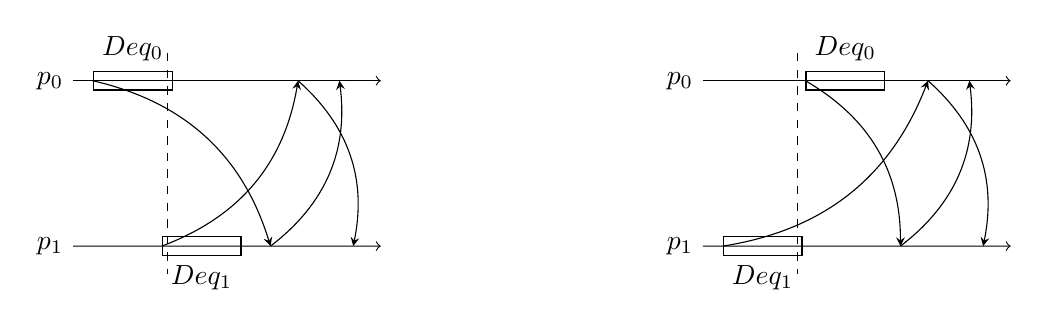
\begin{tikzpicture}
      \begin{scope}[xshift=-4cm,scale=.7]
        \node (p0) at (-1,0){$p_0$};
        \node (p1) at (-1,-3){$p_1$};
        \draw[->] (p0.east) -- (5,0);
        \draw[->] (p1.east) -- (5,-3);
        
        \node[draw,rectangle, minimum width=1cm,label=above:{$Deq_0$}] (d0) at (.5,0){};
        \node[draw,rectangle, minimum width=1cm,label=below:{$Deq_1$}] (d1) at (1.75,-3){};

        \draw[dashed] (1.125,.5) -- (1.125,-3.5);
        
        \path[-stealth] (d0.west) edge[bend left] (3,-3);
        \path[-stealth] (3,-3) edge[bend right] (4.25,0);
        \path[-stealth] (d1.west) edge[bend right] (3.5,0);
        \path[-stealth] (3.5,0) edge[bend left] (4.5,-3);
      \end{scope}

      \begin{scope}[xshift=4cm,scale=.7]
        \node (p0) at (-1,0){$p_0$};
        \node (p1) at (-1,-3){$p_1$};
        \draw[->] (p0.east) -- (5,0);
        \draw[->] (p1.east) -- (5,-3);
        
        \node[draw,rectangle, minimum width=1cm,label=above:{$Deq_0$}] (d0) at (2,0){};
        \node[draw,rectangle, minimum width=1cm,label=below:{$Deq_1$}] (d1) at (.5,-3){};
        
        \draw[dashed] (1.125,.5) -- (1.125,-3.5);

        \path[-stealth] (d0.west) edge[bend left] (3,-3);
        \path[-stealth] (3,-3) edge[bend right] (4.25,0);
        \path[-stealth] (d1.west) edge[bend right] (3.5,0);
        \path[-stealth] (3.5,0) edge[bend left] (4.5,-3);
      \end{scope}
    \end{tikzpicture}
  \end{center}
  In the run pictured on the left, $Deq_0$ must be $Dequeue(1)$, since it return before $Deq_1$'s invocation, and thus the only valid linearization is $Enqueue(1) \cdot Deq_0 \cdot Deq_1$.  In the run on the right, which is indistinguishable to the two processes, since it differs only in the real time of the two $Dequeue$ invocations and processes have no knowledge of real time, the only valid linearization is $Enqueue(1) \cdot Deq_1 \cdot Deq_0$, so $Deq_1$ must be $Dequeue(1)$.  But $Enqueue(1) \cdot Dequeue(1) \cdot Dequeue(1)$ is not legal, so the assumed algorithm is impossible.  
\end{proof}

\begin{theorem}
  Algorithm~\ref{alg:fifo} is an optimal implementation of a FIFO Queue in an asynchronous, failure-free system.
\end{theorem}

  
%%%%%%%%%%%%%%%
%%%%%%%%%%%%%%%
\section{Asynchronous Out-of-Order Queues}

We next move on to consider how we might be able to get around the lower bound in Lemma~\ref{fifolem:pairfreeLB}.  Relaxation has previously been useful for circumventing lower bounds \cite{TalmageWelch14}, so we consider it here.  The $k$-Out-of-Order relaxed $Dequeue$ is still pair-free, since $Dequeue$ cannot return the same value more than once, but there are more possible return values, many of which are not so order-constrained.  We follow \cite{TalmageWelch14} in using relaxation to split $Dequeue$ instances into two types: ``slow'' $Dequeue$s that behave like those in the FIFO algorithm above, taking $2d$ time to return, and ``fast'' $Dequeue$s which return a value immediately on execution, not waiting for the background coordinating communication that slows down other operations.  To enable the algorithm to do this without violating legality, we partition the set of $k$ values which a $Dequeue$ instance can return and give each process ownership of a disjoint subset.  Then that process can safely $Dequeue$ any of its own elements, knowing that no other process will return them to a $Dequeue$.  When a process runs out of elements, its next $Dequeue$ instance will be slow, as it takes the time to coordinate with other processes to determine its return value.  We use that same time to assign ownership of more values, so that future $Dequeue$ instances at that process can be fast again.

Overall, this means that most $Dequeue$ instances take no time at all for comunication delay, vastly outperforming the unrelaxed queue.  The worst case per-instance cost is identical, but the amortized performance is significantly better.  One interesting aspect of this algorithm, that makes it significantly more complex than just adding relaxation handling as previously done in partially synchronous systems to Algorithm~\ref{alg:fifo} is that we can no longer rely solely on timestamp order for linearization.  Since fast $Dequeue$ instances return instantly, there is no guarantee that timstamp order correctly captures their real-time order.  Thus, we must construct a much more complex linearization order to satisfy real-time order, then prove that it is legal.  We rely on invariants related to value ownership, to ensure that fast instances choose values that will be legal for them to return at their linearization points, even if those are quite differnt than the timestamp order the code actually sees. 

%%%%%%%%%%%%%%%
\subsection{Description}

The asynchronous out of order queue is a relaxation of the existing queue structure that relaxes the specification that the queue can only return the first $Enqueue$ instance in $\rho$ that does not already have a matching $Dequeue(-, val)$ in $\rho$. Instead, it allows for the return of any of the first $K Enqueue$ instances in $\rho$ that do not already have a mathing $Dequeue(-, val)$ in $\rho$. 

The K-OOO queue also adds the behavior of prior claiming of elements for a system we will be referring to as "fast dequeueing". The existing behavior for dequeuing will be refered to as a "slow dequeue", which still utilizes the same behavior of Confirmation Lists to replicate information across the network. At points where processes share information however, there is additional behavior developed that allows processes to mark values in the queue that only they will be able to access, that will require no communication to be dequeued. At the point of execution of a "slow dequeue" if a process has a value that is marked to be dequeued by by that process, and the value that is marked is within the bounds of K, that it is one of the first K values in the queue structure, that value can be removed immediately without establishing a Confirmation List and requiring rounds of inter-process communication. Processes that are not the process that has "claimed" the value will additionally view that at the point of the slow dequeue, there is a labeled element for a fast dequeue from the same process, and remove both values from their local view of the queue, in order to ensure the same veiw of the structure. 

The process of labeling is done by guaranteeing that processes have the same view of the queue at certain points, and utilizing this similar view and invariant calculations to collectively agree on which processes claim which values. Given the processes agree on the ordering of values within the queue, the labeling of the elements and the ordering of slow dequeues, we can prove that fast dequeues do not disrupt the existing behavior of the Queue ADT. 
%%%%%%%%%%%%%%%
\subsection{Algorithm}

Because this algorithm is built on Algorithm~\ref{alg:fifo}, we omit some portions that are identical to those in that algorithm.  For example, the code for handling $Enqueue$ instances is exactly the same as that on lines~\ref{fifoline:invEnq}-\ref{fifoline:finishEnq} of Algorithm~\ref{alg:fifo}, so we omit it here, as well as the helper functions.  The code for handling $Dequeue$ is similar that above, but differentiates fast and slow instances, so we present it here. 

In addition to the functions we used before, we add the following functions, which help with labeling elements for fast $Dequeue$:
\begin{itemize}
\item $lQueue.deqByLabel(p)$: Return and remove the oldest element in $lQueue$ which is labeled for process $p$.
\item $lQueue.deqUnlabeled(ts)$: Return and remove the oldest element in $lQueue$ which has timestamp less than $ts$.
\item $lQueue.unlabeledSize()$: Return the number of unlabeled elements in $lQueue$.
\item $lQueue.labelOldest(p,x)$: Label the $x$ oldest elements in $lQueue$ for process $p$.
\end{itemize}
  

\begin{algorithm}
  \caption{Queue with $k$-Out-of-Order Relaxed $Dequeue$: Handlers for $Dequeue$}\label{alg:relaxed}
  \begin{algorithmic}[1]
    \Function{Dequeue}{}
      \State $Deq_{ts} = updateTS()$
      \If {$localQueue.peekByLabel(p_{i}) \neq \bot$}\label{oooline:checkFast}
        \State $ret = localQueue.deqByLabel(p_i)$ \label{oooline:fastDeq}
        \State send $(Deq_f, ret, i, Deq_{ts})$ to all processes
        \State \Return $ret$ \label{oooline:fastDeqResponse}
      \Else
        \State send $(Deq_s, null, i, Deq_{ts})$ to all processes
      \EndIf
    \EndFunction

    \Function{Receive}{($op, val, inv, Deq_{ts})$ from $p_{inv}$}
      \State $updateTS(Deq_{ts})$
      \If{$Deq_{ts}$ is not in $PendingDequeues$}
        \State $PendingDequeues.insertByTS(createList(Deq_{ts}, p_{inv}$))
      \EndIf
      \State send $(op, val, DeqAck, Deq_{ts}, i, p_{inv})$ to all processes
    \EndFunction

    \Function{Receive}{$(op, val, DeqAck, Deq_{ts}, j, p_{inv})$ from $p_j$}
      \If{$Deq_{ts}$ not in $PendingDequeues$}
        \State $PendingDequeues.insertByTs(createList(Deq_{ts}, p_{inv}))$
      \EndIf
      \State Define $currentConfList$ as the confirmation list in $PendingDequeues$ which has $ts == Deq_{ts}$
      \State $currentConfList.responses[j] = True$
      \State $propagateEarlierResponses(PendingDequeues)$ 
      \For{each $confirmationList$ in $PendingDequeues$, in increasing lexicographic timestamp order}
        \If{all $responses$ in $confirmationList$ are $True$}\label{oooline:localExec}
          \If {$op == Deq_f$}
            \If{$p_i \neq p_{inv}$} $lQueue.remove(val)$\EndIf
          \Else    
            \If {$localQueue.peekByLabel(p_{inv}) \neq \bot$}
              \State $ret = lQueue.deqByLabel(p_{inv})$ \label{oooline:sDeqChooseLabeled}
            \Else
              \State $ret = lQueue.deqUnlabeled(Deq_{ts})$ \label{oooline:sDeqChooseUnlabeled}
            \EndIf
            \State $labelElements(p_{inv})$\label{oooline:label}
            \If{$p_i == p_{inv}$}
              \State \Return $ret$
            \EndIf
          \EndIf 
        \EndIf 
      \EndFor
      \EndFunction
%
      \Function{labelElements}{$p_j$} from \cite{TalmageWelch14}
      \State $y = lQueue.unlabeledSize()$
      \State $lQueue.labelOldest(p_j,x)$, where $x = \min\{\lfloor k/n\rfloor, y\}$\label{oooline:labelOldest}
      \EndFunction
  \end{algorithmic}
\end{algorithm}



%%%%%%%%%%%%%%%
\subsection{Correctness}
For the K-OOO queue, we start with a similar structure of a run $R$ and a linearization $\pi$. The primary difference is that the linearization must be more complex, to deal with fast $Dequeue$ instances.  Several lemmas from Section~\ref{sec:fifoCorrectness} still apply to $Enqueue$ and slow $Dequeue$ instances, though we need to extend them to account for fast $Dequeue$ instances.  Once we deal with linearization, the out of order behavior of these instances does not significantly change the correctness argument, it only expands our access to the structure.

Formally, a fast $Dequeue$ instance is one which passes the check on line~\ref{oooline:checkFast}.  Any $Dequeue$ instance which fails this check is slow.

Let $R$ be an arbitrary, admissible, timed run of Algorithm~\ref{alg:relaxed}

\begin{lemma}
 In $R$, every invocation has a matching response.
\end{lemma}

\begin{proof}
  $Enqueue$ and slow $Dequeue$ instances are exactly as in Algorithm~\ref{alg:fifo}, so we omit the proof here, referring the reader to Lemma~\ref{fifolem:responses}.  Fast $Dequeue$ instances will necessarily generate a return on line~\ref{oooline:fastDeqResponse}.  Thus every invocation has a matching response.
\end{proof}

Since we now have operation instances, we can construct a permutation of all instances in $R$.  We then prove tha this permutation is a valid linearization, which shows the correctness of our algorithm.  We define operation instance timestamps as in the previous section.

\begin{construction}\label{constr:relaxed}
  Construct an order of all operation instances in $R$ as follows:
  \begin{enumerate}
  \item Let $\pi$ be the increasing lexicographic order of all $Enqueue$ and slow $Dequeue$ instances. \label{orderSlow}
  \item For each fast $Dequeue$ $op$, in increasing real-time invocation order, let
    \begin{itemize}
    \item $\rho$ be the subsequence of all $Enqueue$ and slow $Dequeue$ instances which return before $op$'s invocation;
    \item $\sigma$ be the subsequence of all fast $Dequeue$ instances already in $\pi$ which return before $op$'s invocation;
    \item $\tau$ be the subsequence of all $Enqueue$ and slow $Dequeue$ instances invoked after $op$ returns.
    \end{itemize}
    Place $op$ in $\pi$ immediately after the later of the last (in $\pi$) elements of $\rho$ and $\sigma$.\label{orderFast}
  \end{enumerate}
\end{construction}

%Note that there may be $Enqueue$ and slow $Dequeue$ instances in neither $\rho$ nor $\tau$ if they are concurrent with $op$.

We need to prove that this sequence respects the real-time order of all non-overlapping operation instances.  We first note that the subsequence defined in step~\ref{orderSlow} respects real-time order by the argument in Lemma~\ref{fifolem:realTimeOrder}.

\begin{lemma}\label{ooolem:fastDeqOrdering}
  When we place each fast $Dequeue$ instance $op$ in step~ref{orderFast} of Construction~\ref{constr:relaxed}, it precedes, in $\pi$, all elements of $\tau$.
\end{lemma}

\begin{proof}
  First, note that all elements of $\rho$ precede all elements of $\tau$ in $\pi$, by step~\ref{orderSlow}.  Next, we prove that all elements of $\sigma$ also precede all elements of $\tau$ in $\pi$.

  Since every element of $\tau$ is invoked after $op$ returns and every element of $\sigma$ returns before $op$ is invoked, every element of $\sigma$ returns before any elmeent of $\tau$ is invoked.  Thus, an element $op'$ of $\sigma$ only follows an elment of $\tau$ in $\pi$ if some previously-placed fast $Dequeue$ instance (in the $\sigma$ when we placed $op'$) was placed in $\pi$ later than that element of $\tau$.  This argument holds in turn for that previously-placed fast $Dequeue$ instance, repeating all the way back to the first fast $Dequeue$ instance step~\ref{orderFast} placed in $\pi$.  That could only be placed after an instance in $op$'s $\tau$ if a previous one was, but there was no previous one, so neither that first fast $Dequeue$ nor any subsequent one could be placed in $\pi$ after an element of $\tau$.  Thus, $op$ precedes every element of $\tau$ in $\pi$.
\end{proof}

\begin{lemma}
  Construction~\ref{constr:relaxed} respects the real-time order of non-overlapping instances in $R$.
\end{lemma}

\begin{proof}
  Consider any two operation instances $op_1$ and $op_2$ in $R$ which do not overlap in real time.  We break the proof down by cases for whether each of $op_1$ and $op_2$ is a fast $Dequeue$ instance or a slow instace: an $Enqueue$ or slow $Dequeue$.
  \begin{itemize}
  \item Both $op_1$ and $op_2$ are slow instances.  This follows from Lemma~\ref{fifolem:realTimeOrder}.
  \item Both $op_1$ and $op_2$ are fast $Dequeue$ instances.  Order follows by construction.  We place the later, in real time order, of $op_1$ and $op_2$ second, and by the definition of $\sigma$ in step~\ref{orderFast} of Construction~\ref{constr:relaxed}, $op_1$ is in $\sigma$, so we place $op_2$ in $\pi$ after $op_1$.
  \item One of $op_1$ is a fast $Dequeue$ instance, the other is a slow instance.  When we place the fast instance (WLOG, $op_1$) in $\pi$, since $op_1$ and $op_2$ do not overlap, then if $op_2$ precedes $op_1$ in real-time order and was thus in $\rho$, so we place $op_1$ after $op_2$ in $\pi$ .  If $op_1$ precedes $op_2$ in real-time order, then $op_2 \in tau$, and Lemma~\ref{ooolem:fastDeqOrdering} proves that $op_1$ precedes $op_2$ in $\pi$.
  \end{itemize}

  Thus, in all cases, $\pi$ respects the real-time order of $op_1$ and $op_2$, for any pair of instances.
\end{proof}

% Local execution seeing same history is the same as above, restricted to slow instances
% Need to prove that processes agree on labels
% Need to prove that once an element is labeled, it is always legal and never returned at a process for which it is not labeled
% Prove legality: slow dequeues as before, fast dequeues can only happen after local execution of the slow dequeue *at the same process* which labeled them, so they are linearized after that, since instances at the same process cannot overlap.

Now that we have a linearization of all instances in our run, we need to show that the return values the algorithm chooses are legal.  $Enqueue$ and slow $Dequeue$ instances function as in the unrelaxed case, with the only difference being how $Dequeue$ chooses its return values.  Now, it will skip elements labeled for other processes.  Since we label at most $\lfloor n/k\rfloor$ elements per process, this will still leave it choosing from among the $k$ oldest elements in the queue, which is legal by the definition of a relaxed queue.  We begin our legality proof by restating Lemma~\ref{fifolem:prevLocalExec} and its corollary in the context of the relaed queue implementation.  We do not re-prove it, as the proof is fundamentally identical.  We note that, despite removing the return value from its $lQueue$ in line~\ref{oooline:fastDeq}, we still refer to local execution as the code starting when line~\ref{oooline:localExec} passes.

\begin{lemma}
  When a process $p_i$ locally executes any $Dequeue$ instance $op$, for any instance $op'$ with a lexicographically smaller timestamp than $op$, $p_i$ has previously locally executed $op'$.
\end{lemma}

\begin{corollary}\label{ooolem:localExecOrder}
  Each process locally executes all $Dequeue$ instances in increasing lexicographic timestamp order.
\end{corollary}

We can now prove the following invariant of our labeling scheme that will enable us to argue that all $Dequeue$ instances return legal values.

\begin{lemma}\label{ooolem:labelOwner}
  Once an element $x$ is labeled $p_i$, no other process will return $x$ to a $Dequeue$ it invoked.
\end{lemma}

\begin{proof}
  The algorithm chooses $Dequeue$ return values in three places: line~\ref{oooline:fastDeq} at a fast $Dequeue$'s invocation or lines~\ref{oooline:sDeqChooseLabeled}, \ref{oooline:sDeqChooseUnlabeled} in local execution of a fast $Dequeue$ at its invoking process.  The last of these will never return a labeled element, so the claim vacuously holds there.  The first two places a process chooses a return value for a $Dequeue$ instance, it chooses one labeled for the instance's invoking process, and we have the claim.
\end{proof}

We can further observe that the code never removes a label, so once processes label a particular element for $p_i$, they will only remove it as the return value of a $Dequeue$ instance invoked at $p_i$.

\begin{lemma}
  $\pi$ is a legal sequence of operation instance, by the definition of a queue with $k$-Out-of-Order relaxed $Dequeue$.
\end{lemma}

\begin{proof}
  We proceed by induction on $\pi$ and prove the following claim in tandem with and to aid in the primary result:

  \begin{claim}\label{ooolem:safeLabels}
    Any $Dequeue$ instance which labels elements during its local execution (line~\ref{oooline:label}) labels only elements which are among the arguments of the $k$ oldest $Enqueue$ instances in the prefix of $\pi$ ending with that $Dequeue$ instance.
  \end{claim}

  The empty sequence is legal.  We assume that for an arbitrary prefix $\rho \cdot op$ of $\pi$, $\rho$ is legal and Claim~\ref{ooolem:safeLabels} holds for all instances in $\rho$.  We will show that $\rho \cdot op$ is also legal and any element $op$ labels is the argument to one of the first $k$ unmatched $Enqueue$ instances in $\rho \cdot op$.  Let $p_i$ be $op$'s invoking process and proceed by cases on $op$'s operation type:
  \begin{itemize}
  \item $op$ is an $Enqueue$ instance.  Since $Enqueue$ has no return value, $\rho \cdot op$ is always legal.
%
  \item $op$ is a slow $Dequeue$ instance, $op = Dequeue(-,ret)$.  $p_i$ chose $ret$ from its $lQueue$ in either line~\ref{oooline:sDeqChooseLabeled} or \ref{oooline:sDeqChooseUnlabeled}.  If it chose it in line~\ref{oooline:sDeqChooseLabeled}, then it was a labeled element, which means that it was the argument of one of the first $k$ unmatched $Enqueue$ instances in a prefix of $\pi$ before some previous slow $Dequeue$ instance.  By Lemma~\ref{ooolem:labelOwner}, no other process could have returned $ret$, and $p_i$ removes it from its $lQueue$ before returning it, so could not have returned it as the return value of another $Dequeue$ instace, and thus $ret$ is still the argument of one of the first $k$ unmatched $Enqueue$ instances in $\rho$.

    If $p_i$ chose $ret$ in line~\ref{oooline:sDeqChooseUnlabeled} and $ret \neq \bot$, then we know that it chose the argument of an unmatched $Enqueue$ instance in $\rho$, since the algorithm puts only $Enqueue$ arguments in $lQueue$, line~\ref{oooline:sDeqChooseUnlabeled} only returns values with timetamps below $ts(op)$, and Corollary~\ref{ooolem:localExecOrder} implies that $p_i$ has already locally executed any $Dequeue$ instance in $\rho$, removing its return value.  Further, $deqUnlabeled$ chooses the oldest eligible element currently in $lQueue$.  By line~\ref{oooline:labelOldest}, no more than $\lfloor k/n\rfloor$ elements are labeled for each process and there are no elements labeled $p_i$, or it would select a return value in line~\ref{oooline:sDeqChooseLabeled} instead, there are fewer than $k$ labeled elements in $lQueue$, so the oldest unlabeled element is among the $k$ oldest elements in $lQueue$ and thus the argument of one of the $k$ oldest $Enqueue$ instances in $\rho$, and $\rho \cdot op$ is legal.

    If $ret = \bot$, then there were no unlabeled elements in $lQueue$ with timestamp smaller than $ts(op)$, which means there are fewer than $k$ unmatched $Enqueue$ instances in $\rho$, and $\rho \cdot op$ is legal.  By Corollary~\ref{ooolem:localExecOrder}, every process locally executes all $Dequeue$ instances in the same order, applying the same deterministic logic.  The only possible differences are that any $p_j$ may have fewer elements labeled for itself, as it has returned them to fast $Dequeue$ instances which it has not yet locally executed.  These instances do not affect the choice of return value for a slow $Dequeue$, though, so each $p_j$ will delete the same $ret$ when locally executing $op$.  

    Finally, we need to prove that Claim~\ref{ooolem:safeLabels} still holds after each process executes line~\ref{oooline:label}, and that all processes label the same elements for $p_i$.  But this follows by the same logic that tells us that $ret$ was the argument of one of the first $k$ unmatched $Enqueue$ intances in $\rho$, as each process chooses elements to label that are the oldest unlabeled elements in $lQueue$.  Thus, each element labeled in the local execution of $op$ is the argument of one of the first $k$ unmatched $Enqueue$ instances in $\rho \cdot op$.  Since all processes locally executed all $Dequeue$ instances in the same order, each will label the same elements while locally executing $op$.
%
  \item $op$ is a fast $Dequeue$ instance, $op = Dequeue(,-,ret)$.  Since we only label elements for process $p_i$ during local execution of a slow $Deuqeue$ instance $op_\ell$ invoked at $p_i$ and no process can have two pending operation instances at the same time, we know that $op$ is invoked after $op_\ell$ returned, so $op$ linearizes after $op_\ell$.  Thus, by Claim~\ref{ooolem:safeLabels}, $ret$ was the argument of one of the first $k$ unmatched $Enqueues$ in $\pi$ before $op_\ell$, and thus before $op$.  By Lemma~\ref{ooolem:labelOwner}, no other process could have returned $ret$, and $p_i$ removes it from its $lQueue$ before returning it, so could not have returned it as the return value of another $Dequeue$ instace, and thus $ret$ is still the argument of one of the first $k$ unmatched $Enqueue$ instances in $\rho$.
  \end{itemize}
\end{proof}

\begin{theorem}
  Algorithm~\ref{alg:relaxed} is a correct implementation of a queue with $k$-Out-of-Order relaxed $Dequeue$.
\end{theorem}

%%%%%%%%%%%%%%%
\subsection{Complexity}



%%%%%%%%%%%%%%%
%%%%%%%%%%%%%%%
\section{Conclusion}

%%%%%%%%%%
\subsection{Less Relaxation than Number of Processes}
In the case in which the X of out of order is less than the number of processes,there isn’t an order of magnitude benefit to relaxation. The benefit of relaxation is that rather than forcing a wait of 2 times the maximum message delay, the wait can be cut to 2 times the (n-x+1)th slowest message delay. In a close connection system, the benefit is minimal as the difference between the max message delay and the (n-x+1)th is minimal, but in an actualized system with nonstandard message delays, this could have some substantial benefits.


\bibliography{refs.bib}

\end{document}
o
